\section{Гидролиз солей. Буферные растворы. Кислоты и основания по Льюису}

\Def{Гидролиз} -- Обменная реакция между водой и растворенным соединением. Так как вода -- амфотерное соединение (в зависимости от условий проявляет кислотные или основные свойства), она может как отдавать ионы \ce{H+} основаниям, так и забирать их у кислот.

\subsection{Механизм гидролиза солей}

Гидролиз солей - взаимодействие ионов соли с ионами воды, приводящее к образованию слабого (малодиссоциирующего) электролита.

У солей с водой могут взаимодействовать катионы или анионы. Для составления уравнений гидролиза следует помнить, что в водных растворах присутствуют и катионы водорода \ce{H+} и гидроксид-ионы \ce{OH-}, образующиеся в ходе диссоциации воды:

\ce{H2O <--> H+ + OH-}

\begin{figure}[H]
    \centering
    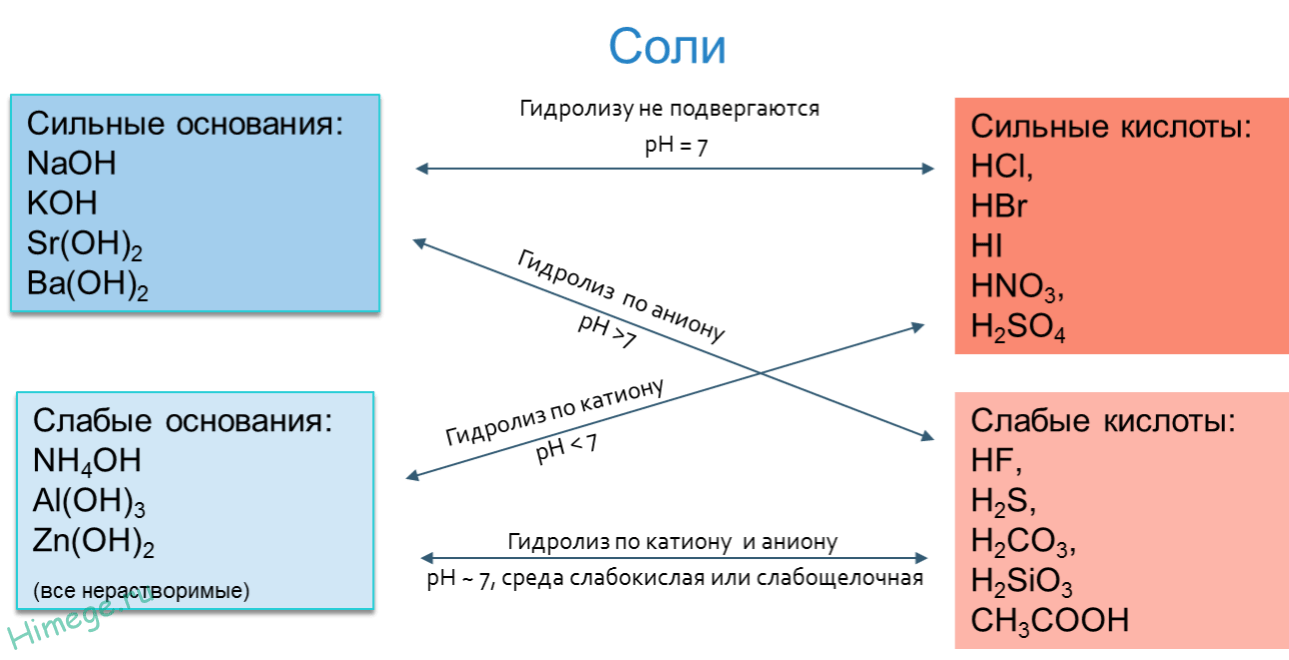
\includegraphics[width = 0.7\textwidth]{TeX/Pictures/17_acidbase.png}
    \caption{Диссоциация кислот и оснований}
    \label{fig:acidbase}
\end{figure}

\subsubsection{Слабое основание + сильная кислота}

В случае, если соль образована слабым основанием и сильной кислотой, она обратимо отдает ион \ce{H+} молекулам воды -- гиддролиз идет по катиону.


\ce{NH4Cl <--> NH4+ + Cl-} -- слабое онование + сильная кислота

\ce{NH4+ + HOH <--> NH4OH + H+} -- выделяются катионы водорода => среда кислая.

\ce{Cl- + HOH} $\neq$  

Итого:

\ce{NH4Cl + H20 <--> NH4OH + HCl}

Гидролиз по катиону, среда кислая (pH<7).

Константу гидролиза можно определить  через ионное произведение воды и константу диссоциации соответствующего катиону основания:

$\displaystyle K_h = \frac{[\ce{NH4OH}][\ce{H+}]}{[\ce{NH4+}]} = \frac{[\ce{NH4OH}][\ce{H+}][\ce{OH-}]}{[\ce{NH4+}][\ce{OH-}]}=\frac{K_\omega}{K_b(\ce{NH4OH})}$

Чем слабее основание(больше $K_b$), тем больше $K_h =>$ сильнее гидролиз соли по катиону.

\subsubsection{Сильное основание + слабая кислота}

\ce{CH3COOK <--> CH3COO- + K+} 

\ce{K+ + HOH} $\neq$

\ce{CH3COO- + HOH <--> CH3COOH + OH-} -- выделяются гидроксид-ионы, среда щелочная.

Итого:

\ce{CH3COOK + H2O <--> CH3COOK + KOH}

Гидролиз по аниону, среда щелочная, (pH>7),

Константу гидролиза по аниону также можно выразить через ионное произведение ыодф и константу диссоциации соответствующей аниону кислоты:

$\displaystyle K_h = \frac{[\ce{CH3COOH}][\ce{OH-}]}{[\ce{CH3COO-}]} = \frac{[\ce{CH3COOH}][\ce{H+}][\ce{OH-}]}{[\ce{CH3COO}][\ce{H+}]}=\frac{K_\omega}{K_a(\ce{CH3COOH})}$

Чем слабее кислота (чем меньше $K_a$, тем больше $K_h =>$ сильнее гидролиз соли по аниону)
\subsubsection{Слабое основание + слабая кислота}

\ce{CH3COONH3 <--> CH3COO- + NH4+}

\ce{CH3COO- + HOH <--> CH3COOH + OH-} -- выделяются гидроксид-ионы.

\ce{NH4Cl <--> NH4+ + Cl-}

\ce{NH4+ + HOH <--> NH4OH + H+} -- выделяются катионы водорода.

Итого:

\ce{CH3COONH4 + H2O <--> CH3COOH + NH4OH}

Гидролиз и по аниону и по катиону, среда нейтральная (pH=7).

\subsubsection{Сильное основание + сильная кислота}

\ce{Na2SO4 <--> 2Na+ + SO4^{2-}}

\ce{Na+ + HOH} $\neq$

\ce{So4^{2-} + HOH} $\neq$

Гидролиз не идет, среда нейтральная (pH=7).
 
 \subsection{Буферные растворы}
 
\begin{wrapfigure}[17]{r}{0.4\textwidth}
  \begin{center}
    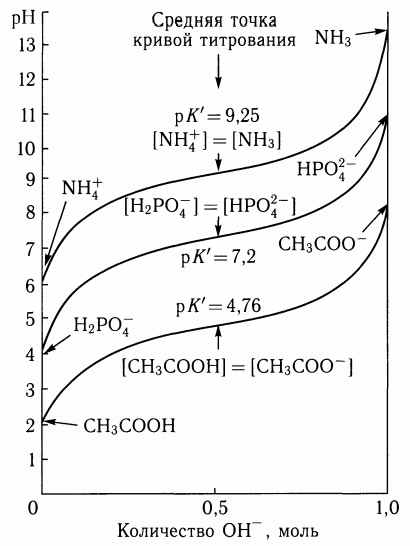
\includegraphics[width=0.38\textwidth]{TeX/Pictures/17_bufcurve.png}
  \end{center}
  \caption{Кривые титрования слабых кислот (\ce{CH3COOH, H2PO4-, NH+}) щелочью}
\end{wrapfigure}
 
 Рассмотрим кривые титрования растворо слабых кислот щелочью (зависимость pH раствора от количества добавленной щелочи). Видно, что в середине всех графиков есть пологий участок в диапазоне $pH = pK_a \pm 1$. То есть при добавлении даже значительного количества щелочи pH изменится слабо. Растворы с такими пропорциями называются буферными. 
 
 \Def{Кислотно-основные буферы} это смесь кислоты \ce{HA} и сопряженного ей основания \ce{A-} или  слабого основания \ce{B} и сопряженной ему кислоты \ce{BH+}
 
 Механизм действия буферной системы:
 
 Если к сопряженной паре \ce{HA}/\ce{A-} добавить сильную кислоту(\ce{H+}), то с ней прореагирует основание \ce{A-}:
 
 \ce{A-  + H+ -> HA}
 
 А если добавить щелочь, ее действие нейтрализуется кислотой \ce{HA}:
 
 \ce{HA + OH- -> A- + H2O}
 
 Кислотность раствора можно найти из концентраций [\ce{A-}] и [\ce{HA}]: $[\ce{H+}] = \frac{K_a[\ce{HA}]}{[\ce{A-}]}$ 
 
 \begin{equation}
     \text{Уравнение Гендерсона-Хассельбаха: }  pH = pK_a + \lg\frac{[\ce{A-}]}{[\ce{HA}]} 
 \end{equation}
 
 

\subsection{Кислоты и основания по Льюису}

\Def{Основания Льюиса} – это доноры пары электронов (все анионы, аммиак и амины, вода, спирты, галогены).

\Def{Кислоты Льюиса} – это акцепторы пары электронов, т.е. соединения, имеющие вакантную орбиталь (ион водорода и катионы металлов: \ce{H+, Ag+, Na+, Fe^{2+}}; галогениды элементов второго и третьего периодов \ce{BF3, AlCl3, FeCl3, ZnCl2}; галогены; соединения олова и серы: \ce{SnCl4, SO3}).

\begin{equation}
\ce{BF3 + F- ->}[\ce{BF4}]    
\end{equation}


\begin{figure}[H]
    \centering
    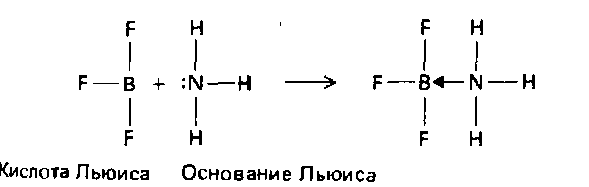
\includegraphics{TeX/TeX_Files/17_luis.png}
    \caption{Взаимодействие основания и кислоты Льюиса — образование связи по донорно-акцепторному механизму}
    \label{fig:luis}
\end{figure}